
%%%%%%%%%%%%%%%%%%%%%%% file typeinst.tex %%%%%%%%%%%%%%%%%%%%%%%%%
%
% This is the LaTeX source for the instructions to authors using
% the LaTeX document class 'llncs.cls' for contributions to
% the Lecture Notes in Computer Sciences series.
% http://www.springer.com/lncs       Springer Heidelberg 2006/05/04
%
% It may be used as a template for your own input - copy it
% to a new file with a new name and use it as the basis
% for your article.
%
% NB: the document class 'llncs' has its own and detailed documentation, see
% ftp://ftp.springer.de/data/pubftp/pub/tex/latex/llncs/latex2e/llncsdoc.pdf
%
%%%%%%%%%%%%%%%%%%%%%%%%%%%%%%%%%%%%%%%%%%%%%%%%%%%%%%%%%%%%%%%%%%%


\documentclass[runningheads,a4paper]{llncs}

\usepackage{amssymb}
\setcounter{tocdepth}{3}
\usepackage{graphicx}
\usepackage{float}
\usepackage{subfigure}

\usepackage{pgfplots}
\usepackage{url}
\usepackage{enumitem}
\usepackage[linesnumbered,ruled]{algorithm2e}
\usepackage[export]{adjustbox}
\usepackage{xspace}
\usepackage{breqn}



\usepackage{url}
\urldef{\mailsa}\path|behrooz.omidvar-tehrani@univ-grenoble-alpes.fr|
\urldef{\mailsb}\path|{freire.pontes, bento.francisco, tiago.oliveira}@academico.ifrn.edu.br|
\urldef{\mailsc}\path|placido.neto@ifrn.edu.br|    
\newcommand{\keywords}[1]{\par\addvspace\baselineskip
\noindent\keywordname\enspace\ignorespaces#1}

\begin{document}

\mainmatter  % start of an individual contribution

% first the title is needed
\title{Highlighting regions preferences from intersection of polygons over time}

% a short form should be given in case it is too long for the running head
\titlerunning{Highlighting region preferences from intersection of polygons over time}

% the name(s) of the author(s) follow(s) next
%
% NB: Chinese authors should write their first names(s) in front of
% their surnames. This ensures that the names appear correctly in
% the running heads and the author index.
%
\author{Pl\'acido A. Souza Neto \and Behrooz Omidvar-Tehrani \and \\
Tiago Oliveira Lisboa \and Francisco B. Silva Junior \and Felipe F. Pontes }
%
\authorrunning{Souza Neto, Pl\'acido A. \textit{et al.}}
% (feature abused for this document to repeat the title also on left hand pages)

% the affiliations are given next; don't give your e-mail address
% unless you accept that it will be published
\institute{Federal Institute of Rio Grande do Norte (Brazil)\\
\mailsc\\
\mailsb\\
University of Grenoble Alpes (France)\\
\mailsa\\}

%
% NB: a more complex sample for affiliations and the mapping to the
% corresponding authors can be found in the file "llncs.dem"
% (search for the string "\mainmatter" where a contribution starts).
% "llncs.dem" accompanies the document class "llncs.cls".
%

\toctitle{Lecture Notes in Computer Science}
\tocauthor{Authors' Instructions}
\maketitle


\begin{abstract}

Many systems consider space and time information. Discover patterns and provide tendencies in spatiotemporal data applications may improve insights for planning and decision making for smart city solutions. Find spatial and temporal preferences can imply to offer interactive and guidance solutions.  For example,  when users look for a house or hotel to spend a season, they consider one or more regions of their preference. These regions are intrinsic to each user. However, when navigating the application, the user also considers regions that seem interesting, for different reasons, such as the priority of some tourist spot, restaurants, clubs, security, etc. Thus, capturing region preferences from mouse tracking over time can help applications to guide the user to find better places. We consider DBSCAN\cite{Ester:1996} and ST-DBSCAN\cite{Birant:2007} algorithms to tackle this challenge, in order to extend GeoGuide \cite{Omidvar:2017} approach, an interactive guidance approach for spatial data, by capturing and saving region preferences in order to highlight informations that can be important and consider to the user.

\keywords{Polygons, mouse-tracking, implicit preferences, regions}
\end{abstract}


\section{Introduction}

%During spatial data analysis, it is often the case that analysts look at some regions of interest but forget to provide an explicit feedback. For instance in Example~\ref{ex:airbnb}, while Liam is focusing on home-stays close to the Eiffel tower, he also looks at farther locations with easy train access. However, he never clicks on those points. 

%We call this latent signal, {\em gaze}. It shown in \cite{fischer1999investigation} that gaze has a strong correlation with ``user attention''. The signal can be captured by tracking eye movements aka saccades~\cite{arapakis2014user}. We employ {\sc ixLabs} gaze tracking\footnote{\it http://www.xlabsgaze.com/} as it only needs a simple web-cam to capture the gaze signal.
 %{\bf Cursor Tracking.} To address privacy issues of web-cam exploitation for gaze tracking, we consider an alternative option of tracking the mouse cursor. It is shown in \cite{arapakis2014understanding} that mouse gestures have a strong correlation with ``user engagement''. Intuitively, a point receives a positive feedback if the cursor moves around it frequently.
 %{\bf Session Time.} In most spatial datasets, there is a profile page dedicated to each point. Examples are restaurant pages in Yelp and lodging pages in Airbnb. We consider the amount of time that the analyst spends in a page as an implicit feedback. For instance, if the analyst spends few minutes in a page for an Indian cuisine restaurant, this counts as positive feedback for this type of restaurants. 

In spatialtemporal data analysis, it is often the case that analysts look at some regions of interest but forget to provide an explicit feedback. To capture user preferences is necessary go beyond filling in attributes and data provided by the user. It is important to understand the user behaviour while using the application to infer about his possible preferences.

\cite{Robertson2007}  affirms that temporal change in spatial patterns are increasingly common in geographical analysis. The work explore an approach to the spatial–temporal analysis of polygons that are spatially distinct and experience discrete changes though time. It presents challenges considering changes of regions (polygons) during the time.

It is shown in \cite{arapakis2014understanding} that mouse gestures have a strong correlation with ``user engagement''. Intuitively, a point receives a positive feedback if the cursor moves around it frequently. We consider privacy issues by tracking the mouse cursor for each user and we consider the mouse movements an explicit user feedback. In most spatial datasets, there is a profile page dedicated to each point. Examples are restaurant pages in Yelp and lodging pages in Airbnb. We consider the amount of time that the user spends in a page as an implicit feedback. For instance, if the user spends few minutes in a page for an Hungary cuisine restaurant or in a page for an apartment with 2 room and garage, this counts as positive feedback for this type of restaurants.

\begin{example}
\label{ex:benicio}
\textit{Ben\'icio} is planning to live a season in Paris. He decides to rent a home-stay from Airbnb website\footnote{\it http://www.airbnb.com}. As he already know the city, because he has a;ready visited several times before decide to spend a season for study. He is open to any type of lodging, considering the regions of his preferences, and he wants to explore his options very carefully. He queries all available locations in Paris with a fair price, although he prefers to live in a more central area of the city, to take better advantage of what Paris can offer. His query results in 3000 locations. As he has no other preferences, an exhaustive investigation needs scanning each location independently which is nearly infeasible. In case he wants to focus on a smaller set of options, it is not clear which subset he needs to look at. While he is looking at primary locations in the list, he shows interest in having ``balcony'' as amenity and being close to Eiffel tower. An ideal system can capture this feedback through mouse-tracking, for instance, in order to short-list a small subset of remaining locations that \textit{Ben\'icio} should consider as high priority based on the regions  which he searched through the mouse movement made on the map of Paris. 
\end{example}

It is shown in \cite{arapakis2014understanding} that mouse gestures have a strong correlation with ``user engagement''. Intuitively, a point receives a positive feedback if the cursor moves around it frequently. We consider privacy issues by tracking the mouse cursor for each user. We consider the mouse movements an implicit user feedback. In most spatial datasets, there is a profile page dedicated to each point. Examples are restaurant pages in Yelp and lodging pages in Airbnb. We consider the amount of time that the user spends in a page as also an implicit feedback. For instance, if the user spends few minutes in a page for an Hungary cuisine restaurant or in a page for an apartment with 2 room and garage, this counts as positive feedback for this type of restaurants.

Figura X apresenta uma sequencia de mapas de Paris mostrando a evolução de como pode ser capturada as regioes de preferencia de Benício, atraves de captura de movimento do mouse. 

\begin{figure} % Inicia o ambiente de figuras
\centering
  \subfigure[Paris map.]{ % Começa a incluir a figura fig1.pdf
   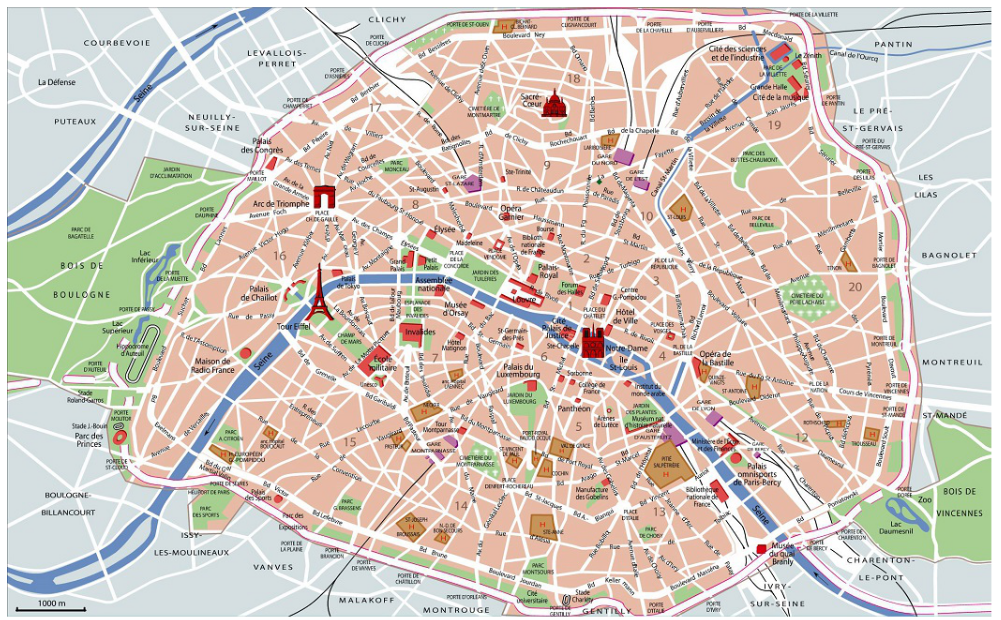
\includegraphics[width=5.8cm]{imgs/adbis2_map0.png}
  \label{fig:paris0} 
  } % Termina de incluir a figura fig1.pdf
  \subfigure[Clusters - time t1.]{ % Começa a incluir a figura fig2.pdf na mesma linha da figura fig1.pdf
    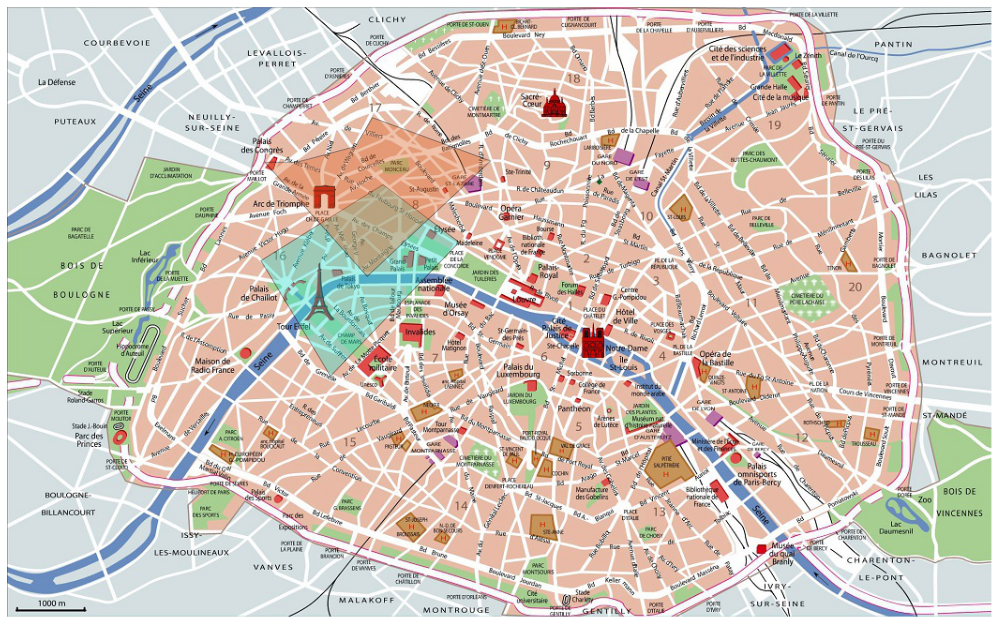
\includegraphics[width=5.8cm]{imgs/adbis2_map1.png}
   \label{fig:paris1}
  } % Termina de incluir a figura fig2.pdf
  \\ % Com esse comando iremos incluir a última figura na próxima linha
  \subfigure[Clusters - time t2.]{ % Começa a incluir a figura fig3.pdf na linha abaixo
    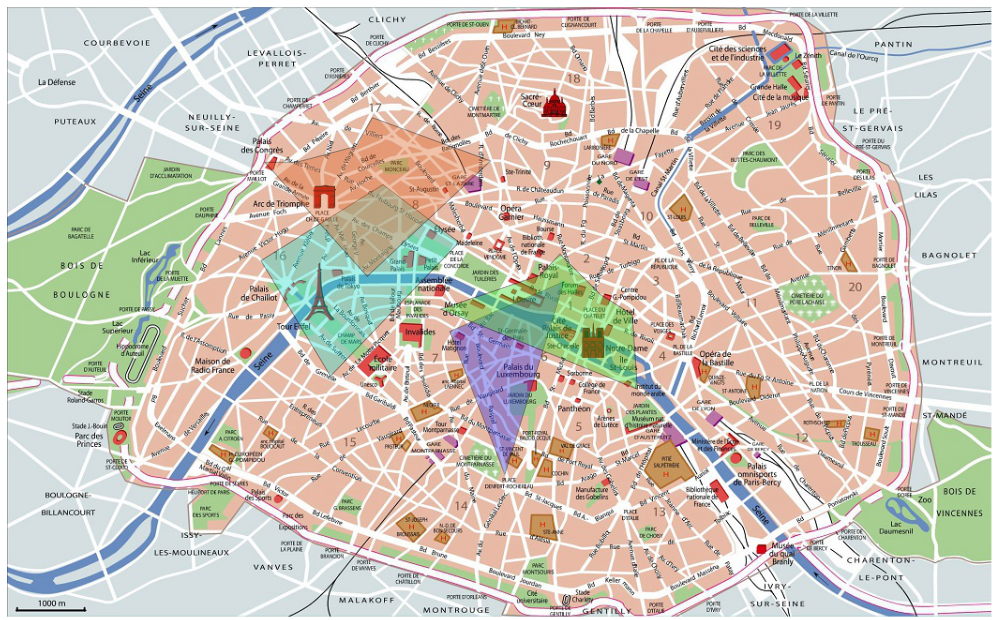
\includegraphics[width=5.8cm]{imgs/adbis2_map2.png}
     \label{fig:paris2} 
  } % Termina de incluir a figura fig3.pdf
   \subfigure[Clusters - time t3.]{ % Começa a incluir a figura fig2.pdf na mesma linha da figura fig1.pdf
    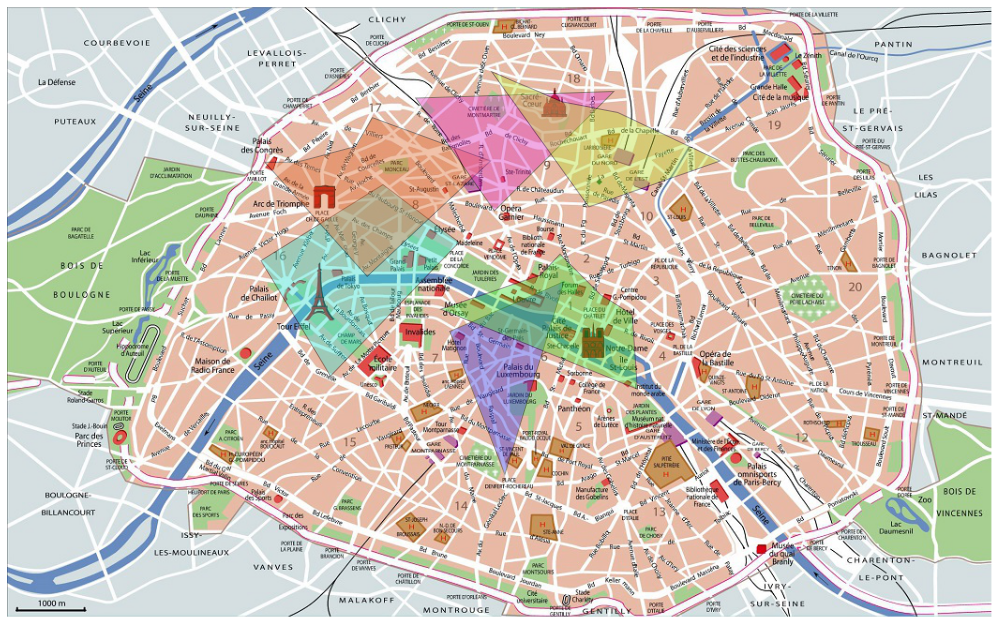
\includegraphics[width=5.8cm]{imgs/adbis2_map3.png}
       \label{fig:paris3} 
  } % Termina de incluir a figura fig2.pdf
  \\ % Com esse comando iremos incluir a última figura na próxima linha
  \subfigure[Intersection of regions.]{ % Começa a incluir a figura fig3.pdf na linha abaixo
    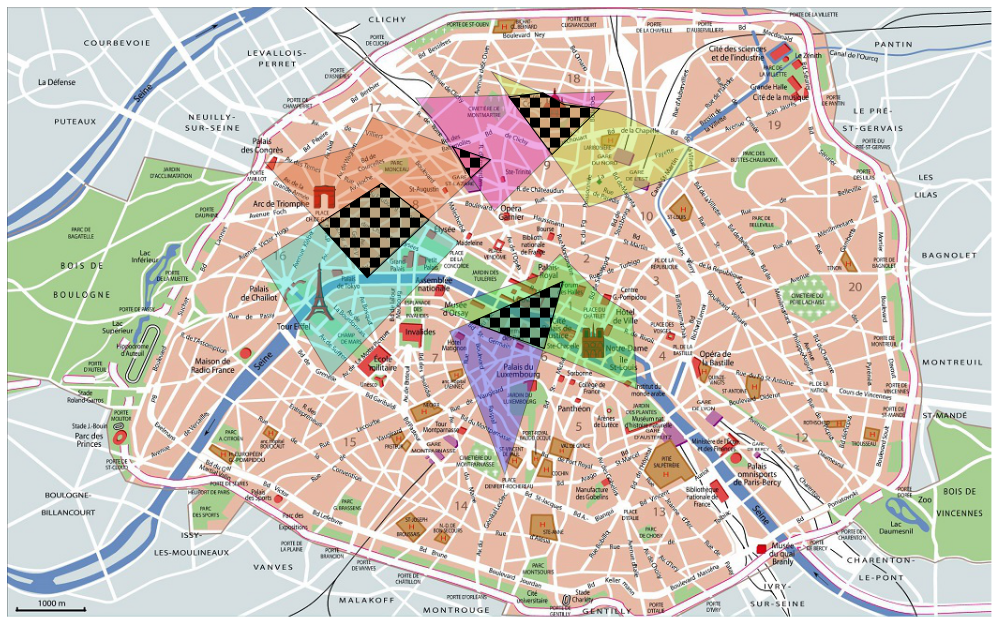
\includegraphics[width=5.8cm]{imgs/adbis2_map4.png}
       \label{fig:paris4} 
  } % Termina de incluir a figura fig3.pdf
   \subfigure[Highlighted regions.]{ % Começa a incluir a figura fig2.pdf na mesma linha da figura fig1.pdf
    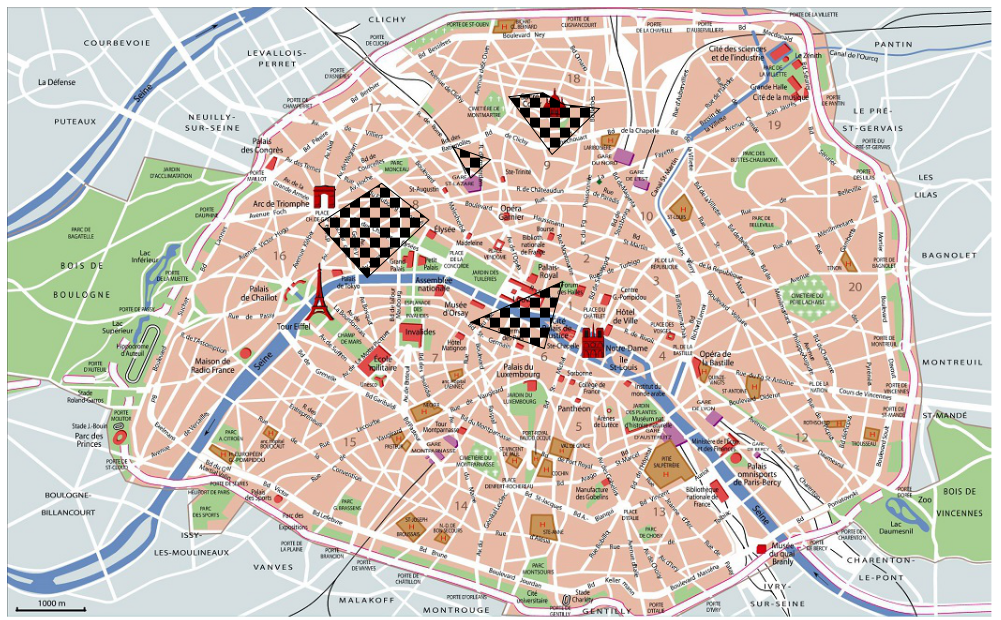
\includegraphics[width=5.8cm]{imgs/adbis2_map5.png}
      \label{fig:paris5} 
  } % Termina de incluir a figura fig2.pdf
  \\ % Com esse comando iremos incluir a última figura na próxima linha
  \caption{Highlighting preference of regions from mouse tracking. }
\end{figure} % Fecha o ambiente de figuras


\section{Overlapping Polygons by Clustering Spatiotemporal Data}
\label{sec:overpolygons}

This section presents some definitions and concepts in order to describe (\textit{i}) how the polygons are created,(\textit{ii}) in which delay of time the set of polygons are grouped, (\textit{iii})  why and how the polygons are overlapped and  (\textit{iv}) how the regions of preferences over time are defined.

Given a dataset of spatial points and from the mouse tracking movements from the user, our approach generates a set of highlighted regions based on its preferences. Each region is related with a subset highlighted points which are illustrated using visual variables such as size and color intensity. The regions are also highlighted.

\noindent {\bf Data Model.} We consider a spatiotemporal database ${\cal D}$ consisting $\langle {\cal R},  {\cal P}, {\cal A},  \rangle$ where ${\cal R}$ is the set of regions, ${\cal P}$ is the set of
geographical points contained in the regions, and ${\cal A}$ is the set of point attributes.  For each $r \in {\cal R}$,  it contains a set of $p \in {\cal P}$, where $p_1,p_2,...,p_n  \in r \land  r \subset	{\cal P}$. We consider a tuple $\langle lat, lon, t\rangle$ where $lat$, $lon$ and $alt$ denote $p$'s geographical coordinates (latitude and longitude  respectively), and $t$ is the timestamp. The set ${\cal A}_p$ contains attribute-values for $p$ over the schema of ${\cal A}$. 

\begin{algorithm}[t]
	\DontPrintSemicolon
	\KwIn{${\cal R}$, $\Delta t \in T$}
	% \KwOut{${\cal S}_p$}
	${ R_p} \gets \emptyset$\;\label{cd:definereturn}
	%$p_{next} \gets get\_next(\mathit{{\cal L}^p})$\;\label{cd:getnext}
	\For{$(r \in {\cal R})$}{\label{cd:beginfr}
		\For{$(r^' \in {\cal R})$}{
			\If{$(r \cap r' \neq \emptyset \wedge get\_time(r) \subseteq t \wedge get\_time(r') \subseteq t $}{\label{cd:if_intersectino}
				${ R_p} \gets  (r \cap r') \wedge { R_p}  $\;
			}
		}
	}
	%	$p_{next} \gets get\_next({\cal L}_p)$\;}\label{cd:endwhile}
	\Return{${ R_p}$}\; 
	\caption{Regions Intersection Algorithm}
	\label{algo:intersectionAlgo}
\end{algorithm}

%For instance, on a bike-sharing dataset, ${\cal A}_p = \langle${\tt female}, {\tt young}, {\tt hybrid-bike}$\rangle$ on the schema ${\cal A} = \langle${\tt gender}, {\tt age}, {\tt type}$\rangle$ denotes that $p$ is associated to a young female cyclist who rides a hybrid bike. The set ${\cal A}$ is domain-dependent and defines the semantics of a spatiotemporal dataset.





\section{Case Study: A GeoGuide Application}

\section{Experiments}


\section{Conclusion}





\vspace{-5pt}

\bibliographystyle{abbrv}
\bibliography{main}

\end{document}
